\hypertarget{introduction-to-coupled-calculations}{%
\section{Introduction to coupled
calculations}\label{introduction-to-coupled-calculations}}

This chapter provides an overview of coupled calculations. Readers who
have already conducted coupled calculations or are familiar with such
calculations can skip this chapter.

First, the physical aspects of a coupled calculation are described. The
weather/climate is formed through the interaction of multiple physical
elements, such as the atmosphere and ocean. For example, momentum from
the atmosphere to the ocean surface and sensible heat from the ocean
surface to the lower boundary of the atmosphere are transported().
Therefore, in a simulation model expressing these phenomena, it is
necessary to exchange physical quantities corresponding to them. At this
time, each model executes a calculation on an appropriate grid system
and time scale according to the physical phenomena represented by the
model. Therefore, to exchange data between models having mutually
different grid systems and time scales, appropriate time management and
grid remapping are required.

\begin{figure}
\hypertarget{fig:ao_interaction}{%
\centering
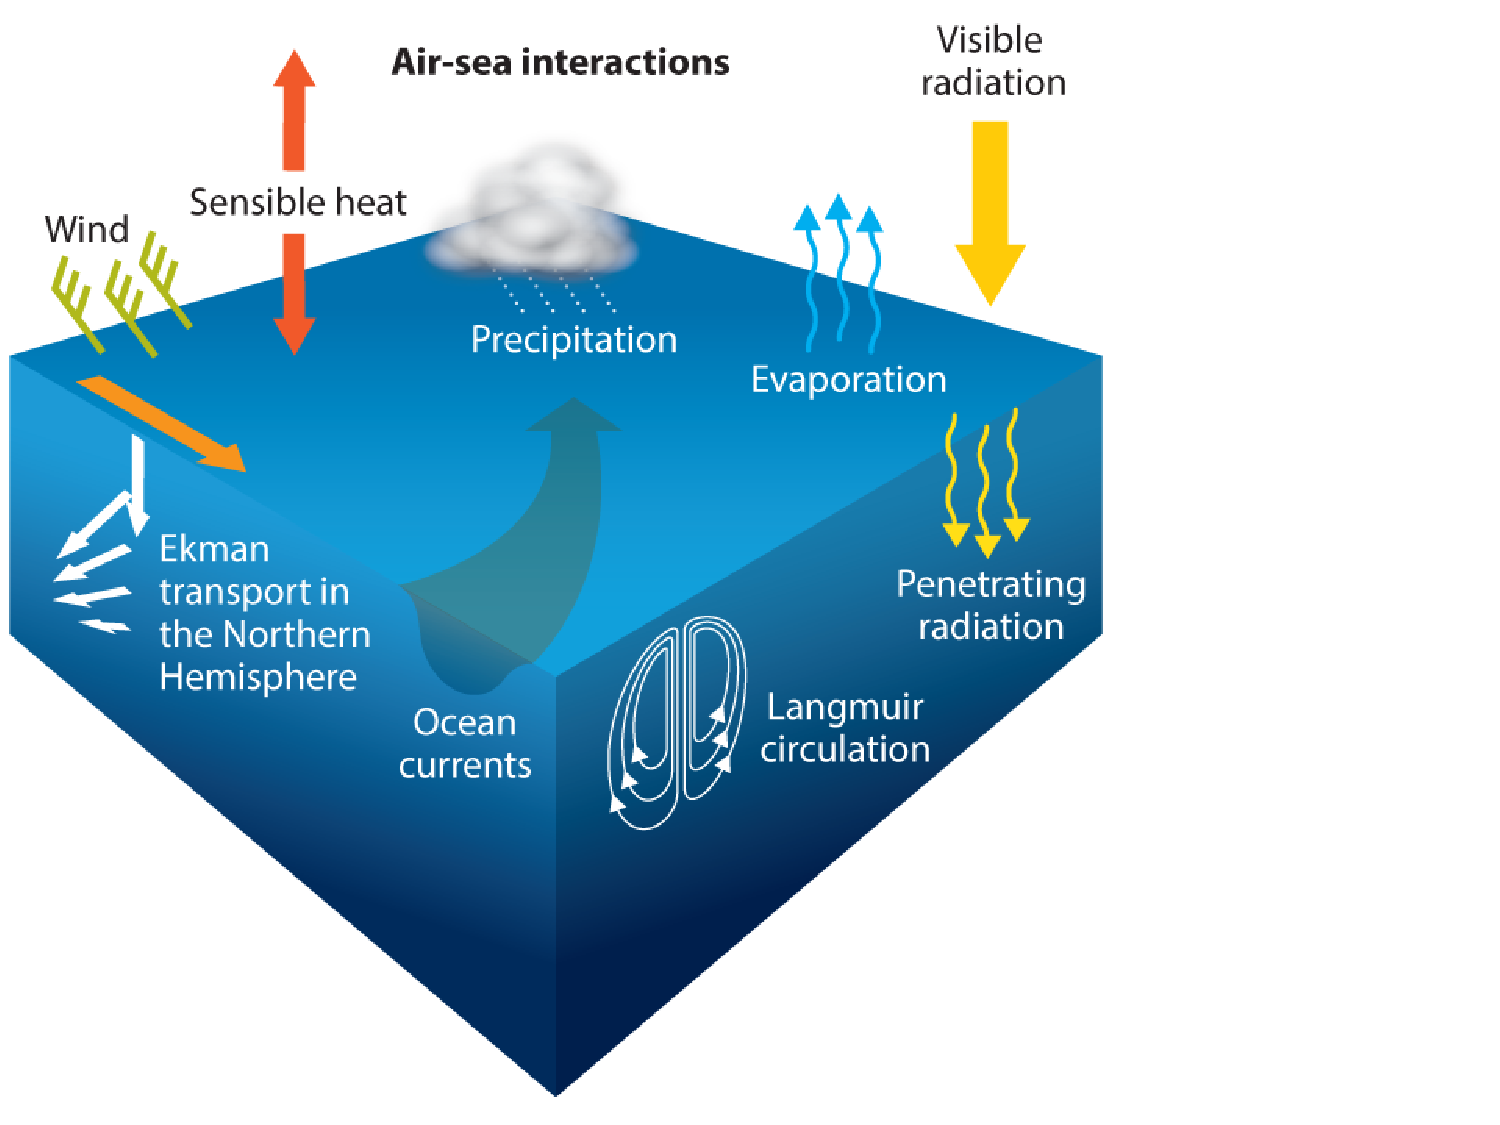
\includegraphics{figs/ao_interaction.pdf}
\caption{Schematics of Atmosphere-Ocean interaction(from Encyclopedia of
the Environment,
https://www.encyclopedie-environnement.org/en/air-en/biosphere-hydrosphere-and-cryosphere-models/)}\label{fig:ao_interaction}
}
\end{figure}

Next, a computational aspect of a coupled calculation is described.
Modern high-performance computers operate a plurality of arithmetic
units in parallel. When running a simulation model on a high-performance
computer, the model must correspond to the architecture of such a
computer. This correspondence is generally realized through a domain
decomposition that divides the model grid. In addition, in a coupled
calculation, a plurality of models are executed in parallel. Therefore,
when exchanging data, it is necessary to conduct a data exchange between
appropriate processes in consideration of a domain decomposition. shows
an example of such a data exchange. Here, it is assumed that model A has
an 8 × 8 grid, and model B has a 12 × 12 grid, and is divided into 4 × 4
and 3 × 3 regions, respectively. Each region is numbered as shown in the
figure. As indicated by the light green arrow, region 5 of model A
exchanges data with regions 0, 1, 3, and 4 of model B. By contrast, as
indicated by the dark green arrows, region 4 of model B exchanges data
with regions 6, 7, 10, and 11 of model A.

It is inappropriate to make individual software for conducting such a
complex data exchange for each model, and therefore dedicated software
for performing a coupled calculation is generally used. This software is
called a coupler or a coupling library.

As mentioned above, there are three main tasks for a coupler:

\begin{enumerate}
\def\labelenumi{\arabic{enumi}.}
\item
  Control of data exchange timing
\item
  Grid remapping
\item
  Data exchange between appropriate processes
\end{enumerate}

\begin{figure}
\hypertarget{fig:data_exchange_example}{%
\centering
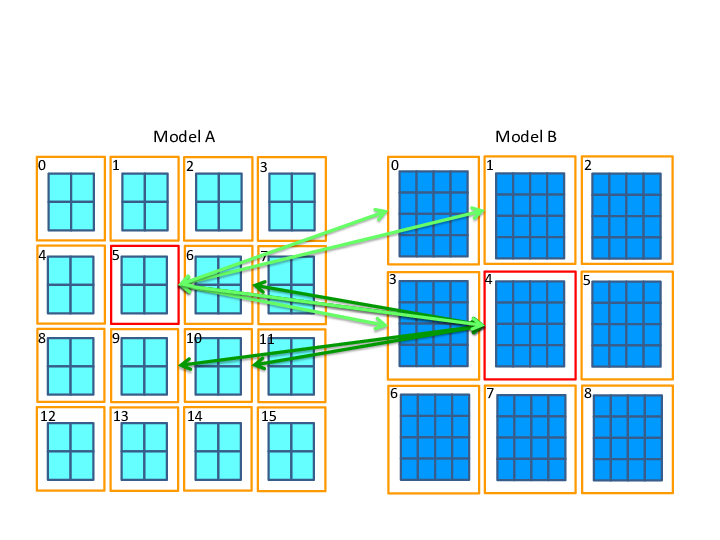
\includegraphics{fig_cpl/data_exchange_example.png}
\caption{Schematic image of data exchange between domain decomposed
models.}\label{fig:data_exchange_example}
}
\end{figure}

\hypertarget{introduction-to-ils-coupling}{%
\section{Introduction to ILS
coupling}\label{introduction-to-ils-coupling}}

\hypertarget{about-ils-coupling-system}{%
\subsection{About ILS Coupling System}\label{about-ils-coupling-system}}

An ILS is composed of multiple component models, such as a land surface
model, MATSIRO; a river model, CaMa-Flood; and a water resources model,
HO8. To couple these component models, an ILS uses Jcup as a coupling
library. Jcup is a general-purpose coupling library, and there are
almost no restrictions on its applicable grid systems and coupling
patterns. However, owing to its high flexibility, its interface is
complicated, making it difficult for beginners to use. Therefore, a
wrapper MOJ (MATSIRO Over Jcup) with a more compact interface customized
to an ILS was developed. MOJ features common to Jcup are summarized as
follows.

\begin{itemize}
\item
  An arbitrary number of two or more components can be coupled
\item
  Each component can be coupled in series or in parallel
\item
  Each component is parallelized through a domain decomposition
\item
  Any grid system can be applied when it has a uniquely numbered grid
\item
  One component model can have multiple grid systems
\item
  An exchange time interval can be set for all data
\item
  Unlimited number of exchangeable data
\item
  Multiple data can be sent and received together based on the
  configuration
\end{itemize}

A user can couple one component model with another by calling the MOJ
API subroutines from the model and setting the configuration file.

\hypertarget{coupling-overview}{%
\subsection{\#\# Coupling Overview}\label{coupling-overview}}

\hypertarget{communicator}{%
\subsubsection{Communicator}\label{communicator}}

Hereinafter, it is assumed that each component model uses an MPI and is
parallelized through a domain decomposition. A parallel program based on
an MPI executes parallel calculations with reference to a communicator.
The default communicator is MPI\_COMM\_WORLD, and there is no problem
using this default communicator when running on a single model. However,
when models are coupled using an MOJ, the communicator of each model is
generated by the MOJ, and it is therefore necessary to change the
communicator to one given by the MOJ. shows a communicator when the
component is used alone and a communicator when coupled with an MOJ. For
a single component, MPI\_COMM\_WORLD is used in all component processes.
By contrast, when coupled with an MOJ, MPI\_COMM\_WORLD is defined for
all processes of all coupled components, and the communicator of each
component is given by the MOJ. The communicator of each component can be
obtained through the MOJ API routine described later.

\begin{figure}
\hypertarget{fig:moj_mpi_comm}{%
\centering
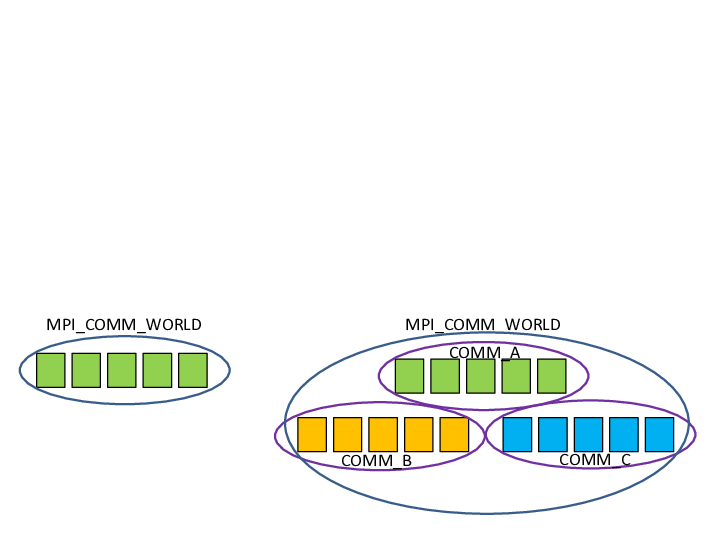
\includegraphics{fig_cpl/moj_mpi_comm.png}
\caption{MPI communicator with components alone and that coupled with an
MOJ (left figure; components alone; right figure; components coupled
with an MOJ)}\label{fig:moj_mpi_comm}
}
\end{figure}

\hypertarget{coupling-pattern}{%
\subsubsection{Coupling Pattern}\label{coupling-pattern}}

An MOJ can combine two (or more) coupled models in series and in
parallel. Here, serial refers to a case in which two components pass
data during the same time step, and parallel refers to a case in which
two components pass data of a previous time step to each other. A
schematic diagram of both patterns is shown in . The left figure is a
serial coupling example, in which the calculation result of model A is
passed to model B during the same time step, and the calculation of
model B is conducted. In serial coupling, each model component waits for
the end of the calculation of the other component, and thus the overall
execution time is substantially equal to the sum of the execution times
of the two components. The right figure shows an example of a parallel
coupling, where the model component sends the calculation result to the
other side component at each time step, and receives the data of the
other side component at the next time step. In this case, the overall
execution time is approximately equal to the time of the component with
the longest execution time. The gray squares before \(T_0\) indicate the
initial value exchange.

\begin{figure}
\hypertarget{fig:coupling_pattern}{%
\centering
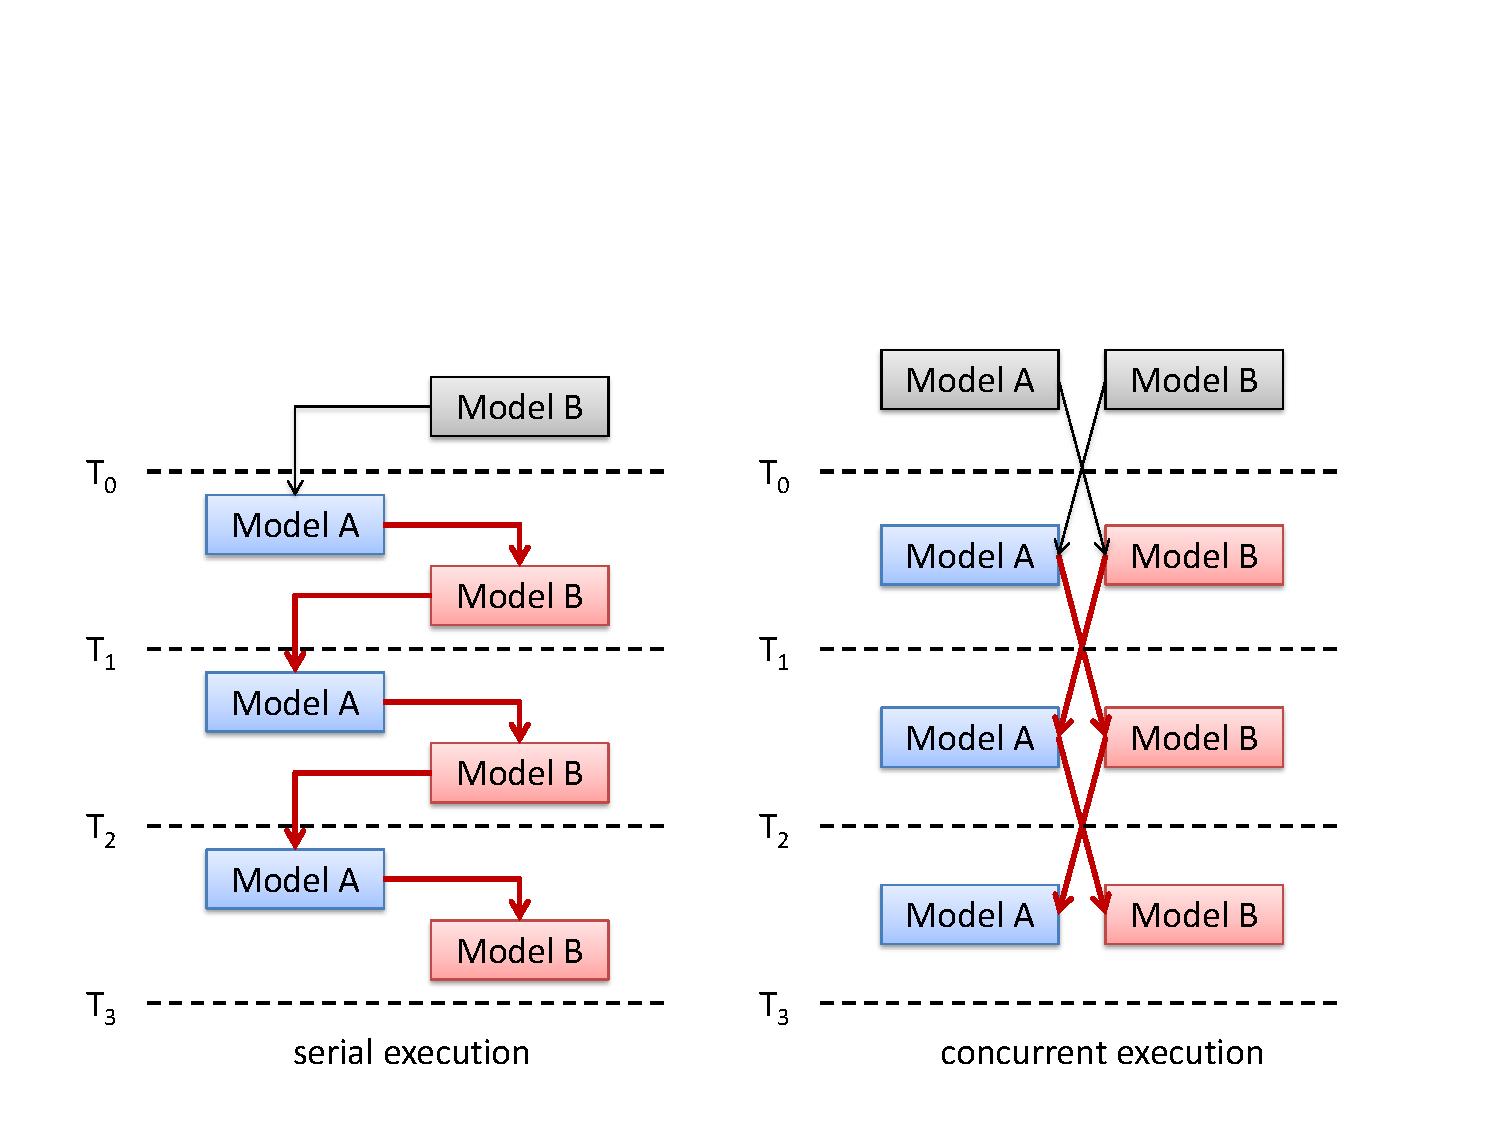
\includegraphics{figs/coupling_pattern.pdf}
\caption{Coupling pattern(left:serial coupling,right:parallel
coupling)}\label{fig:coupling_pattern}
}
\end{figure}

\hypertarget{data-exchange}{%
\subsubsection{Data Exchange}\label{data-exchange}}

The data exchange time interval can be set for each data. In the example
shown in , model B exchanges data with model C every four steps, and
model A every five steps. At the time of a data exchange, each model
requires that the model time coincide with the data exchange time. Time
steps other than the data exchange time do not need to be constant.

\begin{figure}
\hypertarget{fig:data_exchange_pattern}{%
\centering
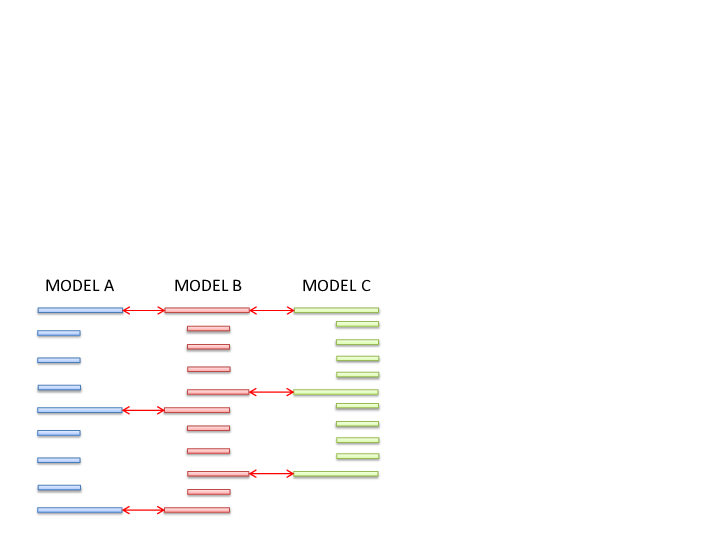
\includegraphics{fig_cpl/data_exchange_pattern.png}
\caption{Data exchange pattern}\label{fig:data_exchange_pattern}
}
\end{figure}

\hypertarget{preparation}{%
\section{Preparation}\label{preparation}}

\hypertarget{grid-index-table}{%
\subsection{Grid index table}\label{grid-index-table}}

Which region (MPI process) of the target component to which all grid
point data are exchanged is determined by the grid point index assigned
to each area of the component model and the mapping table described in
the next section.

The grid point index of the grid assigned to each region is given to the
coupler by the MOJ API subroutine moj\_def\_grid. The index must be made
up of natural numbers. In addition, it does not need to be continuous,
and a discrete number can be applied.

However, the numbers need to be unique among the grid points of all
regions. Because the coupler does not check for duplicate numbers, an
operation in the presence of duplicate grid points cannot be predicted.
One component can have a plurality of grids, and the number of grid
points and the grid point index of each grid can be set independently.

\hypertarget{mapping-table}{%
\subsection{Mapping table}\label{mapping-table}}

An MOJ does not depend on the grid structure and can flexibly couple the
models whose grid does not change over time. However, for this purpose,
it is necessary to obtain the correspondence between grid indexes among
the models and the interpolation coefficients in advance. For example,
as shown in , the value of grid point R(p) of the receiving model is
calculated from grid points \(S(i)-S(i+4)\) and coefficient
\(Cs(i)-Cs(i+4)\), as shown the equation below:

\[R(p) = \sum_{n=0}^{4} Cs(i+n)*S(i+n)\]

The mapping table for \(R(p)\) can be expressed as . For the vector
quantity, a coefficient expressing rotation is further added. These
values are given as arguments of the MOJ API subroutine
moj\_set\_interpolation\_table to be described later.

\begin{figure}
\hypertarget{fig:interpolation_image}{%
\centering
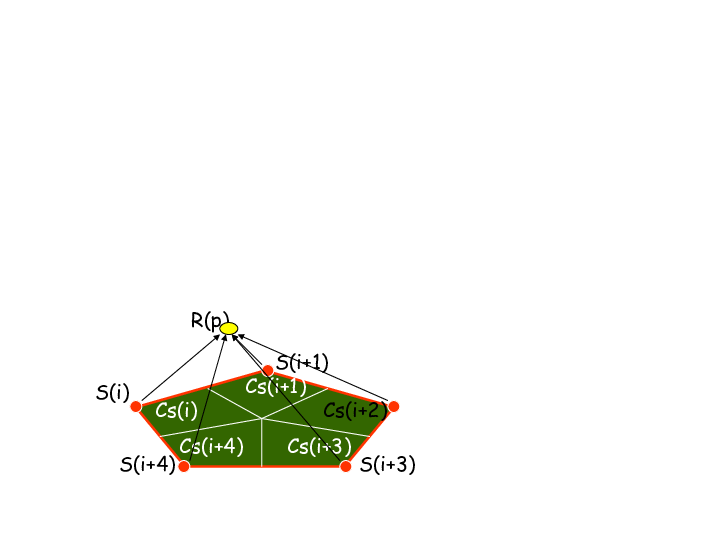
\includegraphics{fig_cpl/interpolation_image.png}
\caption{Grid points and coefficients on interpolation
calculation}\label{fig:interpolation_image}
}
\end{figure}

\hypertarget{list:mapping_table_sample}{%
\label{list:mapping_table_sample}}%
\begin{verbatim}
R(p), S(i), Cs(i)
 R(p), S(i+1), Cs(i+1)
 R(p), S(i+2), Cs(i+2)
 R(p), S(i+3), Cs(i+3)
 R(p), S(i+4), Cs(i+4)
\end{verbatim}

\hypertarget{configuration-file}{%
\subsection{Configuration file}\label{configuration-file}}

To define the operation of an MOJ, it is necessary to create a
configuration file in advance. The name of the configuration file is
given by the MOJ API subroutine moj\_init. What users need to set in the
configuration file are the coupler\_config session, which specifies the
operation of the coupler, and the nam\_moj session, which defines the
exchange data. The elements, descriptions, and possible values for each
session are summarized in and .

The session coupler\_config consists of two elements, log\_level and
debug\_mode. Of these, log\_level sets the detailedness (amount) of the
log output. Possible values include "SILENT," "WISPER," and "LOUD." The
latter value outputs a more detailed log. Debug\_mode is a flag
indicating whether to output a log. If debug\_mode = .false., a log is
not output regardless of the log\_level setting. Note that log\_level =
"LAUD" outputs a large number of logs, and thus care must be taken when
performing long-term integration.

The session nam\_moj describes the sending/receiving components, the
grid, and the data group exchanged between these components. A plurality
of data can be set for a pair of components and a grid, and all data are
interpreted as corresponding to the component and the grid described
immediately before. Settings that can be omitted are shown in italics in
the table.

Var\_put and var\_get are exchange data names, and var\_put\_vec and
var\_get\_vec are exchange vector data names. Either a scalar data name
or a vector data name must be specified. Mapping\_tag is a tag for
specifying a mapping table. Time\_intpl\_tag is a data identification
tag for time interpolation, and data with the same numbered tag are
passed to the time interpolation subroutine of the IO component. This
tag is valid only when coupling IO components. Grid\_intpl\_tag is a
data identification tag for spatial interpolation, and data with the
same number are exchanged as a set of data and passed to the spatial
interpolation subroutine. Intvl sets the data exchange interval in
seconds. Lag sets the coupling pattern. When two components are coupled
in parallel, a value of -1 is given to both the sending and receiving
data, and when they are coupled in series, a value of 1 is given to the
preceding component and a value of -1 is given to the succeeding
component. In addition, 0 indicates a special setting, and is set only
when the initial data are acquired from the IO component using the API
subroutine moj\_get\_initial\_data described later. Layer is an integer
indicating the number of vertical layers of data. Flag is a flag
indicating whether to calculate the time average internally, and
specifies "SNP" or "AVR." Factor is a real constant that is multiplied
with the data at the spatial interpolation. Is\_ok is a flag indicating
whether a data exchange is actually conducted. If is\_ok = 1, the data
are exchanged, and if the value is 0, the data are not exchanged. A
sample of the configuration file is shown in .

\protect\hypertarget{table:coupler_config}{}{{[}table:coupler\_config{]}}

\hypertarget{table:coupler_config}{}
\begin{longtable}[]{@{}lll@{}}
\caption{Elements of couple\_config session of configuration
file}\tabularnewline
\toprule
element name & description  & possible values\tabularnewline
\midrule
\endfirsthead
\toprule
element name & description  & possible values\tabularnewline
\midrule
\endhead
log\_level & log output level & one of "SILENT," "WISPER,"
"LOUD"\tabularnewline
debug\_mode & Flag to output log or not & .true. or
.false.\tabularnewline
\bottomrule
\end{longtable}

\protect\hypertarget{table:nam_moj_comp}{}{{[}table:nam\_moj\_comp{]}}

\hypertarget{table:nam_moj_comp}{}
\begin{longtable}[]{@{}lll@{}}
\caption{Example of nam\_moj section (component and grid
setting)}\tabularnewline
\toprule
element name & description & possible value\tabularnewline
\midrule
\endfirsthead
\toprule
element name & description & possible value\tabularnewline
\midrule
\endhead
comp\_put & sending component name & string of the component
name\tabularnewline
comp\_get & receiving component name & string of the component
name\tabularnewline
grid\_put & grid name of the sending component & string of the grid
name\tabularnewline
grid\_get & grid name of the receiving component & string of the grid
name\tabularnewline
\bottomrule
\end{longtable}

\protect\hypertarget{table:nam_moj_var}{}{{[}table:nam\_moj\_var{]}}

\hypertarget{table:nam_moj_var}{}
\begin{longtable}[]{@{}lll@{}}
\caption{Example of nam\_moj section (exchange data
setting)}\tabularnewline
\toprule
element name & description  & possible value\tabularnewline
\midrule
\endfirsthead
\toprule
element name & description  & possible value\tabularnewline
\midrule
\endhead
var\_put & send data name & string of the name\tabularnewline
var\_get & receive data name & string of the name\tabularnewline
var\_put\_vec & send vector data name & string of the
name\tabularnewline
var\_get\_vec & receive vector data name & string of the data
name\tabularnewline
\emph{mapping\_tag} & mapping table tag & integer for specifying the
mapping table\tabularnewline
\emph{time\_intpl\_tag} & time interpolation tag & integer for
identifying the data\tabularnewline
\emph{grid\_intpl\_tag} & spacial interpolation tag & integer for
identifying the data\tabularnewline
intvl & data exchange interval & integer in second\tabularnewline
lag & coupling pattern & -1 or 0 or 1\tabularnewline
\emph{layer} & number of vertical layer & integer for vertical layer
(default 1)\tabularnewline
flag & time averaging flag & "SNP" or "AVR"\tabularnewline
\emph{factor} & value multiplied to the data & real(kind=8) (default
1)\tabularnewline
\emph{is\_OK} & flag to exchange the data or not & 1 or 0 (default
1)\tabularnewline
\bottomrule
\end{longtable}

\hypertarget{list:moj_namelist_sample}{%
\label{list:moj_namelist_sample}}%
\begin{verbatim}
&coupler_config
  log_level = "LOUD"
  debug_mode  = .true.
&end


&nam_moj  comp_put = "MATIO",   comp_get = "MATSIRO",
          grid_put ='io_grid', grid_get ='matsiro_grid', /
&nam_moj  var_put = 'SWdown'    ,  var_get ='SWdown'    , time_intpl_tag = 1, grid_intpl_tag = 1, intvl=3600 ,  lag=-1, flag='SNP' /
&nam_moj  var_put = 'LWdown'    ,  var_get ='LWdown'    , time_intpl_tag = 2, grid_intpl_tag = 1, intvl=3600 ,  lag=-1, flag='SNP' /
&nam_moj  var_put = 'Rainf'     ,  var_get ='Rainf'     , time_intpl_tag = 2, grid_intpl_tag = 1, intvl=3600 ,  lag=-1, flag='SNP' /
\end{verbatim}

\hypertarget{how-to-use-the-api-subroutines}{%
\section{How to use the API
subroutines}\label{how-to-use-the-api-subroutines}}

\hypertarget{overview-of-their-usage}{%
\subsection{Overview of their usage}\label{overview-of-their-usage}}

To use the MOJ component model, make the API module moj\_api available
in the use statement. A typical usage of the MOJ API routine is as
follows: . First, initialize the MOJ with moj\_init, and make various
settings related to the MPI. Next, various information of the MPI set by
the MOJ is acquired by moj\_get\_comm\_local and moj\_get\_irank\_local.
Set the grid point index of each area of the component with
moj\_def\_grid, and notify the MOJ of the end of the setting with
moj\_end\_grid\_def. Set the mapping table with
moj\_set\_interpolation\_table and give the initial time to the MOJ with
moj\_init\_time. Provide the initial value with moj\_put\_data if
necessary. Finally, tell the MOJ about the end of the join with
moj\_finalize.

\begin{figure}
\hypertarget{fig:moj_usage_sample}{%
\centering
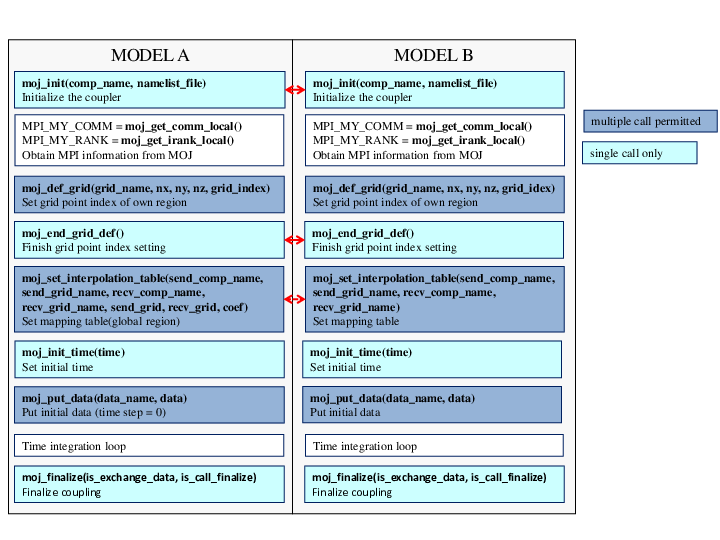
\includegraphics{fig_cpl/moj_usage_sample.png}
\caption{Typical usage of MOJ API routines during the initialization
phase}\label{fig:moj_usage_sample}
}
\end{figure}

The call and internal operation of the MOJ API in the time integration
loop are as shown in . There are three API routines used in the time
integration loop: moj\_set\_time, moj\_get\_data, moj \_put\_data. Call
moj\_set\_time near the beginning of the time integration loop and give
the current time and \(\Delta{T}\) to the MOJ. Data exchange and
interpolation calculations are conducted inside this routine. Obtain the
data of the target component with moj\_get\_data, execute the
calculation, and pass the result to the MOJ with moj\_put\_data. It
should be noted that these API routines must be called for every time
step.

\begin{figure}
\hypertarget{fig:moj_time_integ}{%
\centering
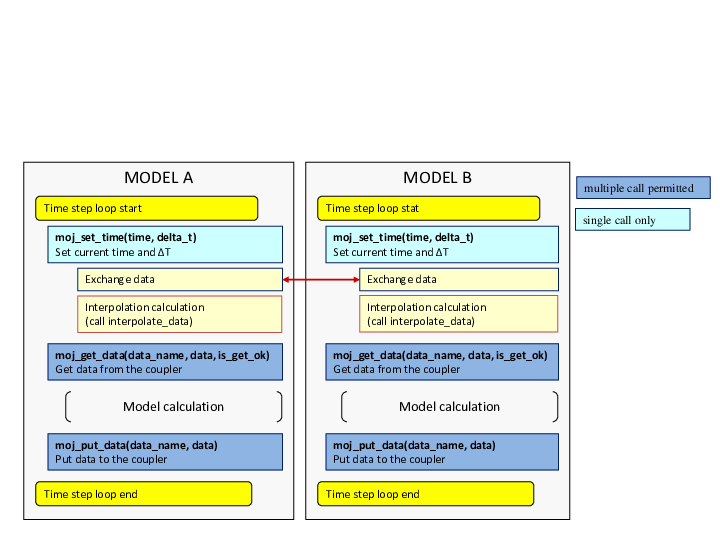
\includegraphics{fig_cpl/moj_time_integ.png}
\caption{Typical usage of MOJ API routines in the time integration
loop}\label{fig:moj_time_integ}
}
\end{figure}

\hypertarget{initialize-moj}{%
\subsection{Initialize MOJ}\label{initialize-moj}}

First, initialize the MOJ with moj\_init. The arguments are the name of
the component and the name of the configuration file. If the MPI
initialization subroutine MPI\_Init is not called in the model
component, it is called inside this routine. Note that calling MPI\_Init
on the model component after calling moj\_init will result in a double
call error.

\hypertarget{get-mpi-information}{%
\subsection{Get MPI information}\label{get-mpi-information}}

As shown by , the MPI communicator of each component when coupled by the
MOJ is generated inside the MOJ. Therefore, the communicator used when a
component calls an MPI routine must be the one generated by the MOJ. The
communicator generated by the MOJ can be obtained using the API function
moj\_get\_comm\_local. In addition, the process number inside the
component can be obtained from the MOJ API routine.

\hypertarget{set-grid-index}{%
\subsection{Set grid index}\label{set-grid-index}}

Set the grid point number with moj\_def\_grid. The arguments are a grid
name, a grid size \((nx, ny, nz)\), and a one-dimensional array
grid\_index(:) of the grid point indexes. What should be noted here is
whether to include the vertical dimension in the array of the grid point
indexes to be given. For example, in the case of atmosphere-ocean
coupling, the exchange data are two-dimensional horizontally, and even
if a third dimension exists, in numerous cases, it is not a physical
vertical layer but a quantity such as a category. Further, even when
exchanging data such as atmosphere and chemistry coupling in a physical
three-dimensional space, the grid differs only in the horizontal plane,
and vertical interpolation may not be necessary in certain cases. When
the mapping table is expressed only in the horizontal plane as in these
examples, even if the data to be exchanged have a vertical layer, the
grid index setting is \(nz = 1\), and the size of the grid\_index is
\(nx *ny\). The above is summarized as follows.

\begin{itemize}
\item
  When the exchange data are horizontal 2D data or the interpolation
  calculation is horizontally 2D only

  nz = 1, and grid\_index is given as an array of size \(nx * ny\).
\item
  Interpolation calculation in 3D space including vertical

  grid\_index is given as an array of size \(nx * ny * nz\).
\end{itemize}

When exchanging 3D data including a vertical layer in the former case,
the number of vertical layers is given to the layer by setting
individual data in the setting file.

\hypertarget{set-mapping-table}{%
\subsection{Set mapping table}\label{set-mapping-table}}

The mapping table setting subroutine moj\_set\_interpolation\_table must
be called by both the sending component and the receiving component.
Because a data exchange is conducted inside this subroutine, the calling
location must correspond in the sending and receiving components.
Arguments after the grid point index are optional arguments and are
given by the receiving component. Further, when the data to be exchanged
are only of a scalar amount or there is no rotation of the grid, it is
not necessary to provide two arguments of coef\_sin and coef\_cos. The
above results are shown in .

\protect\hypertarget{table:interpolation_table_arguments}{}{{[}table:interpolation\_table\_arguments{]}}

\hypertarget{table:interpolation_table_arguments}{}
\begin{longtable}[]{@{}lll@{}}
\caption{Arguments of moj\_set\_interpolation\_table}\tabularnewline
\toprule
Arguments & meaning & Criteria to give \tabularnewline
\midrule
\endfirsthead
\toprule
Arguments & meaning & Criteria to give \tabularnewline
\midrule
\endhead
send\_comp\_name & send component name &\tabularnewline
send\_grid\_name & send grid name & give both\tabularnewline
recv\_comp\_name & receive component name & component\tabularnewline
recv\_grid\_name & receive grid name &  \tabularnewline
send\_index & send grid index & give on the\tabularnewline
recv\_index & receive grid index & receive component\tabularnewline
coef & interpolation coefficient &\tabularnewline
coef\_sin & rotation coefficient & give on the receive
component\tabularnewline
coef\_cos & rotation coefficient & and rotation is
necessary\tabularnewline
\bottomrule
\end{longtable}

\hypertarget{set-initial-time}{%
\subsection{Set initial time}\label{set-initial-time}}

Give the initial time with moj\_set\_init\_time. The argument is an
integer array of size 6, representing the year, month, day, hour,
minute, and second.

\hypertarget{initial-value-put}{%
\subsection{Initial value Put}\label{initial-value-put}}

Before entering the time integration loop, the sending side must put the
data received in the first step. The API subroutine is moj\_put\_data or
moj\_put\_data\_vec, and the arguments are the data name and data (one
variable for the scalar data and two variables for the vector data).

\hypertarget{time-integration}{%
\subsection{Time integration}\label{time-integration}}

\hypertarget{setting-of-current-time-and-deltat}{%
\subsubsection{\texorpdfstring{Setting of current time and
\(\Delta{T}\)}{Setting of current time and \textbackslash Delta\{T\}}}\label{setting-of-current-time-and-deltat}}

Call the API routine moj\_set\_time in the time integration loop and
give the current time and \(\Delta{T}\). The arguments are an integer
array of size 6 representing the year, month, day, hour, minute, and
second, and an integer representing \(\Delta{T}\). Note that (currently)
the unit of \(\Delta{T}\) is only in seconds. Because processing inside
the coupler, such as a data exchange determination, uses the integrated
value of \(\Delta{T}\), moj\_set\_time must be called at every step.

\hypertarget{obtaining-the-data}{%
\subsubsection{Obtaining the data}\label{obtaining-the-data}}

To obtain the target data, call moj\_get\_data or moj\_get\_data\_vec.
The argument data\_name is the data name, and data, or data1, data2, is
the receiving data array. The optional argument data\_scalar is a scalar
quantity received at the same time as these data, and the optional
argument data\_scalar must also be given in moj\_put\_data of the
corresponding target component. The optional argument is\_get\_OK is a
logical type argument that returns whether the step is a data receiving
step.

\hypertarget{putting-the-data}{%
\subsubsection{Putting the data}\label{putting-the-data}}

To send data, moj\_put\_data or moj\_put\_data\_vec is called, which is
the same as the initial value, Put. The argument data\_name is the data
name, and data, or data1 and data2, are sending data arrays. The
optional argument data\_scalar is the scalar quantity to be sent at the
same time as these data. If the step is not a sending step, the
processing is appropriately conducted (sending is skipped) inside the
coupler, and thus it is not necessary for the user to make a call
determination according to the step.

\hypertarget{ending-process}{%
\subsection{Ending process}\label{ending-process}}

Finally, moj\_finalize is called at the end of the coupling. The
argument is\_exchange\_data is a flag for sending/receiving the last
step data inside moj\_finalize when the last step data are not
sent/received owing to the time integration step algorithm. Here,
"is\_call\_finalize" is a flag indicating whether to call the MPI
termination routine MPI\_finalize internally.

\hypertarget{other-main-routines}{%
\subsection{Other main routines}\label{other-main-routines}}

\hypertarget{get-initial-value}{%
\subsubsection{Get initial value}\label{get-initial-value}}

The subroutine moj\_get\_initial\_data is used to obtain the initial
value from the IO component. The arguments are a data name and an array
to obtain the data. This subroutine must be called before the time
integration. In addition, it is necessary to set the reading of the
initial value in the configuration file used by the IO component.

\hypertarget{get-mpi-information-1}{%
\subsubsection{Get MPI information}\label{get-mpi-information-1}}

In addition to the communicator acquisition function
moj\_get\_comm\_local, moj\_get\_irank\_local, which returns the rank of
its own component, and moj\_get\_numpe\_local, which returns the number
of ranks, are provided. A subroutine moj\_get\_mpi\_parameter for
obtaining MPI information at a particular time is also provided.

\hypertarget{data-exchange-1}{%
\subsubsection{Data exchange}\label{data-exchange-1}}

Moj\_send\_value and moj\_recv\_value are provided as subroutines for
sending data to and receiving data from the target component. The
argument is a character string comp\_name representing the name of the
target component and a character string, or an integer, an integer
array, a real number, or a real number array, representing a data
exchange.

\hypertarget{calendar-operation-routine}{%
\subsubsection{Calendar operation
routine}\label{calendar-operation-routine}}

A subroutine group for adding/subtracting the date, month, day, hour,
minute, and second according to the type of calendar and calculating the
difference between two times is provided. See the reference for details
regarding this content.

\hypertarget{setting-information-acquisition-routine}{%
\subsubsection{Setting information acquisition
routine}\label{setting-information-acquisition-routine}}

Although not required for normal use of the MOJ, there are routines that
return the settings in the configuration file for special purposes. See
the references for details on the individual routines.

\hypertarget{log-output-routine}{%
\subsubsection{Log output routine}\label{log-output-routine}}

Here, moj\_put\_log outputs a Jcup format log to a Jcup log file. The
argument sub\_name is the name of the subroutine, and log\_str is the
character string of the log.

\hypertarget{execution-information-acquisition-routine}{%
\subsubsection{Execution information acquisition
routine}\label{execution-information-acquisition-routine}}

Here, moj\_is\_coupled is a function that returns whether the component
specified by the argument comp\_name is currently running (coupled).

\hypertarget{references}{%
\section{References}\label{references}}

\hypertarget{apis-of-moj}{%
\subsection{APIs of MOJ}\label{apis-of-moj}}

\hypertarget{public-constants}{%
\subsubsection{Public constants}\label{public-constants}}

The constants published by the MOJ are shown in . These are all
constants for specifying the type of calendar to be used, and are used
as arguments of the API subroutine moj\_init\_calendar described later.
CALENDAR\_NORLAM indicates that a normal Gregorian calendar is used,
CALENDAR\_NOLEAPYEAR uses a calendar fixed at 365 days a year without
leap years, and CALENDAR\_30360 indicates that a calendar is fixed at
360 days a year, and 30 days a month.

\protect\hypertarget{table:moj_constant}{}{{[}table:moj\_constant{]}}

\hypertarget{table:moj_constant}{}
\begin{longtable}[]{@{}ll@{}}
\caption{Public constants of MOJ}\tabularnewline
\toprule
name & description \tabularnewline
\midrule
\endfirsthead
\toprule
name & description \tabularnewline
\midrule
\endhead
CALENDAR\_NORMAL & Use regular Gregorian calendar\tabularnewline
CALENDAR\_NOLEAPYEAR & Use a fixed calendar of 365 days a year without
considering leap years\tabularnewline
CALENDAR\_30360 & Use a fixed calendar of 30 days a month, 360 days a
year\tabularnewline
\bottomrule
\end{longtable}

\hypertarget{initialization-apis}{%
\subsubsection{Initialization APIs}\label{initialization-apis}}

The MOJ API subroutine group related to initialization is shown in .
Subroutine moj\_init initializes the MOJ. The argument is a character
string representing the component name and the configuration file name.
This subroutine is called only once. The subroutine moj\_def\_grid sets
the grid used by each component. The argument grid\_name represents the
name of the grid. In addition, nx, ny, and nz represent the size of the
grid assigned to the area. In a model such as CaMa, which expresses grid
points in one dimension, nx is the given grid size, and ny and nz may be
set to 1. grid\_index is an integer array indicating the grid point
index of the grid in charge of its own area. This subroutine can be
called multiple times depending on the number of grid systems coupled.
The subroutine moj\_end\_grid\_def declares the end of the grid
definition.

The subroutine moj\_set\_interpolation\_table sets the grid point
correspondence and interpolation coefficients used in an interpolation
calculation. The arguments send\_comp\_name, send\_grid\_name,
recv\_comp\_name, and recv\_grid\_name represent a send component name,
a send grid name, a receive component name, and a receive grid name,
respectively. In addition, ``send\_index'' and ``recv\_index'' are the
grid point indexes on the sending and receiving sides in the
interpolation calculation. The correspondence for all regions is given,
and the size of the two arrays must match. Note that this argument may
be given by the route processor of the receiving component. Here, "coef"
is an array corresponding to the interpolation coefficient \(C\) when
calculating \(R = R + S * C\), and "coef\_sin" and "coef\_cos" are
rotation coefficients when the rotating vector quantities are
\(U = u*coef\_cos*u-coef\_sin*v\) and \(V = coef\_sin*u + coef\_cos*v\).
The subroutine moj\_init\_time sets the initial time of the calculation.
The argument time\_array(:) is an integer of size 6 representing the
year, month, day, hour, minute, and second.

Note that these subroutines must be called in the order shown in the
table.

\protect\hypertarget{table:moj_api_initialize}{}{{[}table:moj\_api\_initialize{]}}

\hypertarget{table:moj_api_initialize}{}
\begin{longtable}[]{@{}llll@{}}
\caption{Initialization API of MOJ}\tabularnewline
\toprule
routine name & type of argument & argument  &
description\tabularnewline
\midrule
\endfirsthead
\toprule
routine name & type of argument & argument  &
description\tabularnewline
\midrule
\endhead
moj\_init & & &\tabularnewline
& character(len=*), intent(IN) & comp\_name & component
name\tabularnewline
& character(len=*), intent(IN) & namelist\_file & configuration file
name\tabularnewline
moj\_def\_grid & & &\tabularnewline
& character(len=*), intent(IN) & grid\_name & grid name\tabularnewline
& integer, intent(IN) & nx & number of local grid points\tabularnewline
& & & in i-direction\tabularnewline
& integer, intent(IN) & ny & number of local grid points\tabularnewline
& & & in j-direction\tabularnewline
& integer, intent(IN) & nz & number of local grid points\tabularnewline
& & & in k-direction\tabularnewline
& integer, intent(IN) & grid\_index(:) & grid point index\tabularnewline
& & & of local grid\tabularnewline
moj\_end\_grid\_def & & &\tabularnewline
& no argument & &\tabularnewline
moj\_set\_ & & &\tabularnewline
interpolation\_table & character(len=*), intent(IN) & send\_comp\_name &
send component name\tabularnewline
& character(len=*), intent(IN) & send\_grid\_name & send grid
name\tabularnewline
& character(len=*), intent(IN) & recv\_comp\_name & receive component
name\tabularnewline
& character(len=*), intent(IN) & recv\_grid\_name & receive grid
name\tabularnewline
& integer, optional, intent(IN) & send\_index(:) & grid index
of\tabularnewline
& & & send component\tabularnewline
& integer, optional, intent(IN) & recv\_index(:) & grid index
of\tabularnewline
& & & receive component\tabularnewline
& real(kind=8), optional, intent(IN) & coef(:) & interpolation
coefficient\tabularnewline
& real(kind=8), optional, intent(IN) & coef\_sin(:) & rotation
coefficient(sin)\tabularnewline
& real(kind=8), optional, intent(IN) & coef\_cos(:) & rotation
coefficient(cos)\tabularnewline
moj\_init\_time & & &\tabularnewline
& integer, intent(IN) & time\_array(:) & integar array\tabularnewline
& & & yy/mo/dd/hh/mm/ss\tabularnewline
moj\_get\_initial\_data & & &\tabularnewline
& character(len=*), intent(IN) & data\_name & data name\tabularnewline
& real(kind=8), intent(INOUT) & data(:),data(:,:),data(:,:,:) & receive
data\tabularnewline
& logical, intent(OUT) & is\_get\_ok & receive data flag\tabularnewline
\bottomrule
\end{longtable}

\hypertarget{apis-in-the-time-integration-loop}{%
\subsubsection{APIs in the time integration
loop}\label{apis-in-the-time-integration-loop}}

API subroutines for exchanging data in the time integration loop are
shown in . The subroutine moj\_set\_time is given an integer array of
size 6 representing the current time and an integer representing
\(\Delta{T}\). This subroutine is to be called at the beginning of the
time integration loop, and data exchanges are executed within this
subroutine based on the current time (exactly the elapsed time
calculated by the summation of \(\Delta{T}\)). The subroutines
moj\_put\_data and moj\_put\_data\_vec give scalar or vector data to the
coupler. The subroutines moj\_get\_data and moj\_get\_data\_vec are
subroutines for obtaining scalar or vector data from the coupler. The
optional argument is\_get\_ok is a logical type argument that returns
whether the data were actually acquired when this subroutine was called.
In general, because the data exchange time interval does not match the
time step of the model component, whether the data are acquired at that
time is determined by referring to this argument.

\protect\hypertarget{table:moj_api_integration}{}{{[}table:moj\_api\_integration{]}}

\hypertarget{table:moj_api_integration}{}
\begin{longtable}[]{@{}llll@{}}
\caption{Data exchange APIs}\tabularnewline
\toprule
routine name & type of argument & argument  &
description\tabularnewline
\midrule
\endfirsthead
\toprule
routine name & type of argument & argument  &
description\tabularnewline
\midrule
\endhead
moj\_set\_time & & &\tabularnewline
& integer, intent(IN) & time\_array(:) & current time\tabularnewline
& integer, intent(IN) & delta\_t & \(\Delta{T}\)\tabularnewline
moj\_put\_data & & &\tabularnewline
& character(len=*), intent(IN) & data\_name & data name\tabularnewline
& real(kind=8), intent(IN) & data(:) or data(:,:) or data(:,:,:) & send
data\tabularnewline
& real(kind=8), intent(IN) & scalar\_data & send value\tabularnewline
moj\_put\_data\_vec & & &\tabularnewline
& character(len=*), intent(IN) & data\_name & data name\tabularnewline
& real(kind=8), intent(IN) & data1(:) or data1(:,:) or data1(:,:,:) &
send data 1\tabularnewline
& real(kind=8), intent(IN) & data2(:) or data2(:,:) or data2(:,:,:) &
send data 2\tabularnewline
& real(kind=8), intent(IN) & scalar\_data & send value\tabularnewline
moj\_get\_data & & &\tabularnewline
& character(len=*), intent(IN) & data\_name & data name\tabularnewline
& real(kind=8), intent(INOUT) & data(:) or data(:,:) or data(:,:,:) &
receive data\tabularnewline
& real(kind=8), intent(OUT) & scalar\_data & receive
value\tabularnewline
& logical, intent(OUT) & is\_get\_ok & data receive flag\tabularnewline
moj\_get\_data\_vec & & &\tabularnewline
& character(len=*), intent(IN) & data\_name & data name\tabularnewline
& real(kind=8), intent(INOUT) & data1(:) or data1(:,:) or data1(:,:,:) &
receive data 1\tabularnewline
& real(kind=8), intent(INOUT) & data2(:) or data2(:,:) or data2(:,:,:) &
receive data 2\tabularnewline
& real(kind=8), intent(OUT) & scalar\_data & receive
value\tabularnewline
& logical, intent(OUT) & is\_get\_ok & data receive flag\tabularnewline
\bottomrule
\end{longtable}

\hypertarget{finalize-api}{%
\subsubsection{Finalize API}\label{finalize-api}}

API subroutine for coupling finalization is shown in . The subroutine
moj\_finalize is called at the end of the coupling. The argument
is\_exchange\_data is a flag indicating whether to send and receive data
after the end of the final step, and is set according to the status of
the time step of the component. The argument is\_call\_finalize is a
flag indicating whether to call the MPI finalizing subroutine
MPI\_Finalize in moj\_finalize.

\protect\hypertarget{table:moj_api_finalize}{}{{[}table:moj\_api\_finalize{]}}

\hypertarget{table:moj_api_finalize}{}
\begin{longtable}[]{@{}llll@{}}
\caption{Finalize API}\tabularnewline
\toprule
routine name & type of argument & argument  &
description\tabularnewline
\midrule
\endfirsthead
\toprule
routine name & type of argument & argument  &
description\tabularnewline
\midrule
\endhead
moj\_finalize & & &\tabularnewline
& logical, intent(IN) & is\_exchange\_data & flag of exhcange the data
or not\tabularnewline
& logical, intent(IN) & is\_call\_finalize & flag of calling
MPI\_finalize or not\tabularnewline
\bottomrule
\end{longtable}

\hypertarget{other-apis}{%
\subsubsection{Other APIs}\label{other-apis}}

Although it is possible to couple only the initialization subroutine
group, the time integration subroutine group, and the finalization
subroutine described in the previous section, utility routine groups are
provided to enhance the convenience of the MOJ. The utility routine
groups for each application are described below.

\hypertarget{query-apis-of-mpi-setting}{%
\paragraph{Query APIs of MPI setting}\label{query-apis-of-mpi-setting}}

The functions and subroutines for obtaining MPI information are shown in
. Here, moj\_get\_comm\_local, moj\_get\_irank\_local,
moj\_get\_numpe\_local are functions that return the communicator of the
component, the local rank number, and the total number of local
processes, respectively. In addition, moj\_get\_mpi\_parameter is a
subroutine for collectively acquiring these pieces of MPI information.

\protect\hypertarget{table:moj_api_mpi}{}{{[}table:moj\_api\_mpi{]}}

\hypertarget{table:moj_api_mpi}{}
\begin{longtable}[]{@{}llll@{}}
\caption{MPI setting of query APIs}\tabularnewline
\toprule
routine name & type of argument & argument  & descrition\tabularnewline
\midrule
\endfirsthead
\toprule
routine name & type of argument & argument  & descrition\tabularnewline
\midrule
\endhead
moj\_get\_comm\_local & & &\tabularnewline
& no argument & &\tabularnewline
moj\_get\_irank\_local & & &\tabularnewline
& no argument & &\tabularnewline
moj\_get\_numpe\_local & & &\tabularnewline
& no argument & &\tabularnewline
moj\_get\_mpi\_parameter & & &\tabularnewline
& integer, intent(OUT) & my\_comm & communicator\tabularnewline
& integer, intent(OUT) & my\_group & groupe ID\tabularnewline
& integer, intent(OUT) & my\_size & the number of local
process\tabularnewline
& integer, intent(OUT) & my\_ranki & local rank number\tabularnewline
\bottomrule
\end{longtable}

\hypertarget{apis-for-sendreceive-values}{%
\paragraph{APIs for send/receive
values}\label{apis-for-sendreceive-values}}

A subroutine for sending and receiving data between two components is
shown in . Here, moj\_send\_value sends a string, integer, or real
number to the other components. This subroutine is meaningful only to
the component's root process. In addition, moj\_recv\_value receives a
character string, integer, or real number from the sending component.
This subroutine must be called simultaneously on all processes of the
receiving component. Moreover, sending and receiving need to have a
one-to-one correspondence.

\protect\hypertarget{table:moj_api_sendrecv}{}{{[}table:moj\_api\_sendrecv{]}}

\hypertarget{table:moj_api_sendrecv}{}
\begin{longtable}[]{@{}llll@{}}
\caption{APIs for sending/receiving values}\tabularnewline
\toprule
routine name & type of argument & argument  &
description\tabularnewline
\midrule
\endfirsthead
\toprule
routine name & type of argument & argument  &
description\tabularnewline
\midrule
\endhead
moj\_send\_value & & &\tabularnewline
& character(len=*), intent(IN) & comp\_name & receive component
name\tabularnewline
& character(len=*), intent(IN) & send\_string & send
string\tabularnewline
or & integer, intent(IN) & send\_inteter & send integer\tabularnewline
or & integer, intent(IN) & send\_inteter(:) & send integer
array\tabularnewline
or & real(kind=8), intent(IN) & send\_real8 & send double\tabularnewline
or & real(kind=8), intent(IN) & send\_real8(:) & send double
array\tabularnewline
moj\_recv\_value & & &\tabularnewline
& character(len=*), intent(IN) & comp\_name & send component
name\tabularnewline
& character(len=*), intent(OUT) & recv\_string & receive
string\tabularnewline
or & integer, intent(OUT) & recv\_inteter & receive
integer\tabularnewline
or & integer, intent(OUT) & recv\_inteter(:) & receive integer
array\tabularnewline
or & real(kind=8), intent(OUT) & recv\_real8 & receive
double\tabularnewline
or & real(kind=8), intent(OUT) & recv\_real8(:) & receive double
array\tabularnewline
\bottomrule
\end{longtable}

\hypertarget{calendar-apis}{%
\paragraph{Calendar APIs}\label{calendar-apis}}

The subroutine group related to a calendar calculation is shown in .
Here, moj\_inc\_time adds \(\Delta{T}\) given by moj\_set\_time to the
current time. In addition, moj\_init\_calendar sets the type of
calendar. The argument is one of the constants CALENDAR\_NORMAL,
CALENDAR\_NOLEAPYEAR, or CALENDAR\_30360, published in the API.
Moreover, moj\_inc\_calendar and moj\_dec\_calendar add and subtract
\(\Delta{T}\) to the year, month, day, hour, minute, and second given in
the first argument, and moj\_inc\_month and moj\_dec\_month add and
subtract months in the same way. In addition, moj\_cal\_date\_diff
calculates the difference (second) between two years, months, days,
hours, minutes, and seconds, and moj\_get\_month\_date returns the
number of days in a certain year and month.

\protect\hypertarget{table:moj_api_calendar}{}{{[}table:moj\_api\_calendar{]}}

\hypertarget{table:moj_api_calendar}{}
\begin{longtable}[]{@{}llll@{}}
\caption{APIs for calendar calculation}\tabularnewline
\toprule
routine name & type of argument & argument & description\tabularnewline
\midrule
\endfirsthead
\toprule
routine name & type of argument & argument & description\tabularnewline
\midrule
\endhead
moj\_inc\_time & & &\tabularnewline
& integer, intent(INOUT) & time\_array(6) & array of
yy/mo/dd/hh/mm/ss\tabularnewline
moj\_init\_calendar & & &\tabularnewline
& integer, intent(IN) & calendar\_type & one of
CALENDAR\_NORMAL,\tabularnewline
& & & CALENDAR\_NOLEAPLEAY,\tabularnewline
& & & CALENDAR\_30360\tabularnewline
moj\_inc\_calendar & & &\tabularnewline
& integer, intent(INOUT) & time\_array(6) & array of
yy/mo/dd/hh/mm/ss\tabularnewline
& integer, intent(IN) & delta\_t & seconds to add\tabularnewline
moj\_dec\_calendar & & &\tabularnewline
& integer, intent(INOUT) & time\_array(6) & array of
yy/mo/dd/hh/mm/ss\tabularnewline
& integer, intent(IN) & delta\_t & senconds to subtruct\tabularnewline
moj\_inc\_month & & &\tabularnewline
& integer, intent(INOUT) & time\_array(6) & array of
yy/mo/dd/hh/mm/ss\tabularnewline
& integer, intent(IN) & delta\_m & months to add\tabularnewline
moj\_dec\_calendar & & &\tabularnewline
& integer, intent(INOUT) & time\_array(6) & array of
yy/mo/dd/hh/mm/ss\tabularnewline
& integer, intent(IN) & delta\_m & months to subtruct\tabularnewline
moj\_cal\_date\_diff & & &\tabularnewline
& integer, intent(IN) & time\_array1(6) & array of
yy/mo/dd/hh/mm/ss\tabularnewline
& integer, intent(IN) & time\_array2(6) & array of
yy/mo/dd/hh/mm/ss\tabularnewline
& integer, intent(OUT) & deff\_sec &
array2-array1(seconds)\tabularnewline
moj\_get\_month\_date & & &\tabularnewline
& integer, intent(IN) & year & year\tabularnewline
& integer, intent(IN) & month & month\tabularnewline
\bottomrule
\end{longtable}

\hypertarget{query-apis-of-configuration}{%
\paragraph{Query APIs of
configuration}\label{query-apis-of-configuration}}

shows the subroutine group for acquiring the setting information. These
are subroutines for acquiring information defined in the configuration
file described in the Preparation section. In each case, the data
exchange interval and the data tag for interpolation calculation are
acquired from the send component name and the data name, or from the
receive component name and the data name.

\protect\hypertarget{table:moj_api_config}{}{{[}table:moj\_api\_config{]}}

\hypertarget{table:moj_api_config}{}
\begin{longtable}[]{@{}llll@{}}
\caption{Query APIs of configuration information}\tabularnewline
\toprule
routine name & type of argument & argument  &
description\tabularnewline
\midrule
\endfirsthead
\toprule
routine name & type of argument & argument  &
description\tabularnewline
\midrule
\endhead
moj\_get\_ & & &\tabularnewline
exchange\_interval\_put & character(len=*), intent(IN) & put\_comp\_name
& send component name\tabularnewline
& character(len=*), intent(IN) & put\_data\_name & send data
name\tabularnewline
& integer, intent(OUT) & intvl & exchange
interval(seconds)\tabularnewline
moj\_get\_ & & &\tabularnewline
exchange\_interval\_get & character(len=*), intent(IN) & get\_comp\_name
& receive component name\tabularnewline
& character(len=*), intent(IN) & get\_data\_name & receive data
name\tabularnewline
& integer, intent(OUT) & intvl & exchange
interval(seconds)\tabularnewline
moj\_get\_grid\_tag\_put & & &\tabularnewline
& character(len=*), intent(IN) & put\_comp\_name & send component
name\tabularnewline
& character(len=*), intent(IN) & put\_data\_name & send data
name\tabularnewline
& integer, intent(OUT) & tag & spacial interpolation tag\tabularnewline
moj\_get\_grid\_tag\_get & & &\tabularnewline
& character(len=*), intent(IN) & get\_comp\_name & receive component
name\tabularnewline
& character(len=*), intent(IN) & get\_data\_name & receive data
name\tabularnewline
& integer, intent(OUT) & tag & spacial interpolation tag\tabularnewline
moj\_get\_time\_tag\_put & & &\tabularnewline
& character(len=*), intent(IN) & put\_comp\_name & send component
name\tabularnewline
& character(len=*), intent(IN) & put\_data\_name & send data
name\tabularnewline
& integer, intent(OUT) & tag & time interpolation tag\tabularnewline
moj\_get\_time\_tag\_get & & &\tabularnewline
& character(len=*), intent(IN) & get\_comp\_name & receive component
name\tabularnewline
& character(len=*), intent(IN) & get\_data\_name & receive data
name\tabularnewline
& integer, intent(OUT) & tag & time interpolation tag\tabularnewline
moj\_get\_get\_comp\_name & & &\tabularnewline
& character(len=*), intent(IN) & put\_comp\_name & send component
name\tabularnewline
& character(len=*), intent(IN) & put\_data\_name & send data
name\tabularnewline
& character(len=*), intent(OUT) & get\_comp\_name & receive component
name\tabularnewline
\bottomrule
\end{longtable}

\hypertarget{log-output-api}{%
\paragraph{Log output API}\label{log-output-api}}

shows the subroutine that outputs a Jcup format log to a Jcup log file.
The argument sub\_name is the name of the subroutine, and log\_str is a
character string to be output.

\protect\hypertarget{table:moj_api_log}{}{{[}table:moj\_api\_log{]}}

\hypertarget{table:moj_api_log}{}
\begin{longtable}[]{@{}llll@{}}
\caption{Log output API}\tabularnewline
\toprule
routine name & type of argument & argument  &
description\tabularnewline
\midrule
\endfirsthead
\toprule
routine name & type of argument & argument  &
description\tabularnewline
\midrule
\endhead
moj\_put\_log & & &\tabularnewline
& character(len=*), intent(IN) & sub\_name & subroutine
name\tabularnewline
& character(len=*), intent(IN) & log\_str & log string\tabularnewline
\bottomrule
\end{longtable}

\hypertarget{execution-information-query-api}{%
\paragraph{Execution information query
API}\label{execution-information-query-api}}

shows the function that returns whether the component specified by the
argument is currently being executed (coupled). The argument comp\_name
is the name of the target component.

\protect\hypertarget{table:moj_api_coupled}{}{{[}table:moj\_api\_coupled{]}}

\hypertarget{table:moj_api_coupled}{}
\begin{longtable}[]{@{}llll@{}}
\caption{API for execution informatioin}\tabularnewline
\toprule
routine name & type of argument & argument  &
description\tabularnewline
\midrule
\endfirsthead
\toprule
routine name & type of argument & argument  &
description\tabularnewline
\midrule
\endhead
moj\_is\_coupled & & &\tabularnewline
& character(len=*), intent(IN) & comp\_name & component
name\tabularnewline
\bottomrule
\end{longtable}
